\chapter{Physics Background}
\section{The Phenomena of Spin}

Spin is a fundamental quantity possessed by all elementary particles. We use
the word 'spin' to describe the property, because partices which possess spin,
behave as though they have some kind of intrinsic, hidden rotation, as if they
were 'spinning'. The dimension of spin, therefore is angular momentum. What is
somewhat bizarre about spin, is that we do not observe anything physically
spinning - although there are some phenomena (such as oribtal angular momenta)
which can be naively thought of as a 'spinning system' (but this description
escapes classical analogy, due to its quantum, probibalistic nature). The role
of Spin in Physics is of foundational importance, and yet, we have not
succesfully produced a model which can accurately predict the spin of hadrons.

The presence of spin in relativistic particles creates the phenomona of
chriality, which has huge implications for how elementary particles can generate
structure in matter itself ~\needcite{}. In the case of the weak interaction,
the presence of spin, which creates Chiral spinors breaks the left-right
symmetry of weak coupling in matter (a fact which will be exploited in this
thesis to probe the spin of the proton sea).

The phenomena of spin also changes the rules for how ensembles of particles may
exist in a potential. Particles with spin are fermions, and because these
paritcles must obey fermi statistics, we can observe structure in matter in the
universe ~\needcite{}. Without spin, the world as we know would collapse on
itself, making any kind of extended non-exotic structures which currenlty exist
by virtue of the Pauli exclusion principal, impossible.

\section{A Brief History of Proton Spin}

The study of Spin is really just an outgrowth of the general study of matter.
Our models for matter, and the underlying structure of matter (in the modern
sense), represents over a hundred years of experimental and theoretical efforts,
and thousands of years of contemplating what makes up the universe.

\subsection{About 2,500 Years Ago...}
Sometime around 490 - 370 BCE lived two philosophers, empedocles
(Fig~\ref{fig:empedocles}), and Democrtius (Fig~\ref{fig:democritus}). Both men
lived approximately at the same time, and made huge philosophical leaps in
attempting to understand the nature of the visible world.

\begin{figure}[H]
	\centering
	\begin{subfigure}{.5\textwidth}
		\centering
		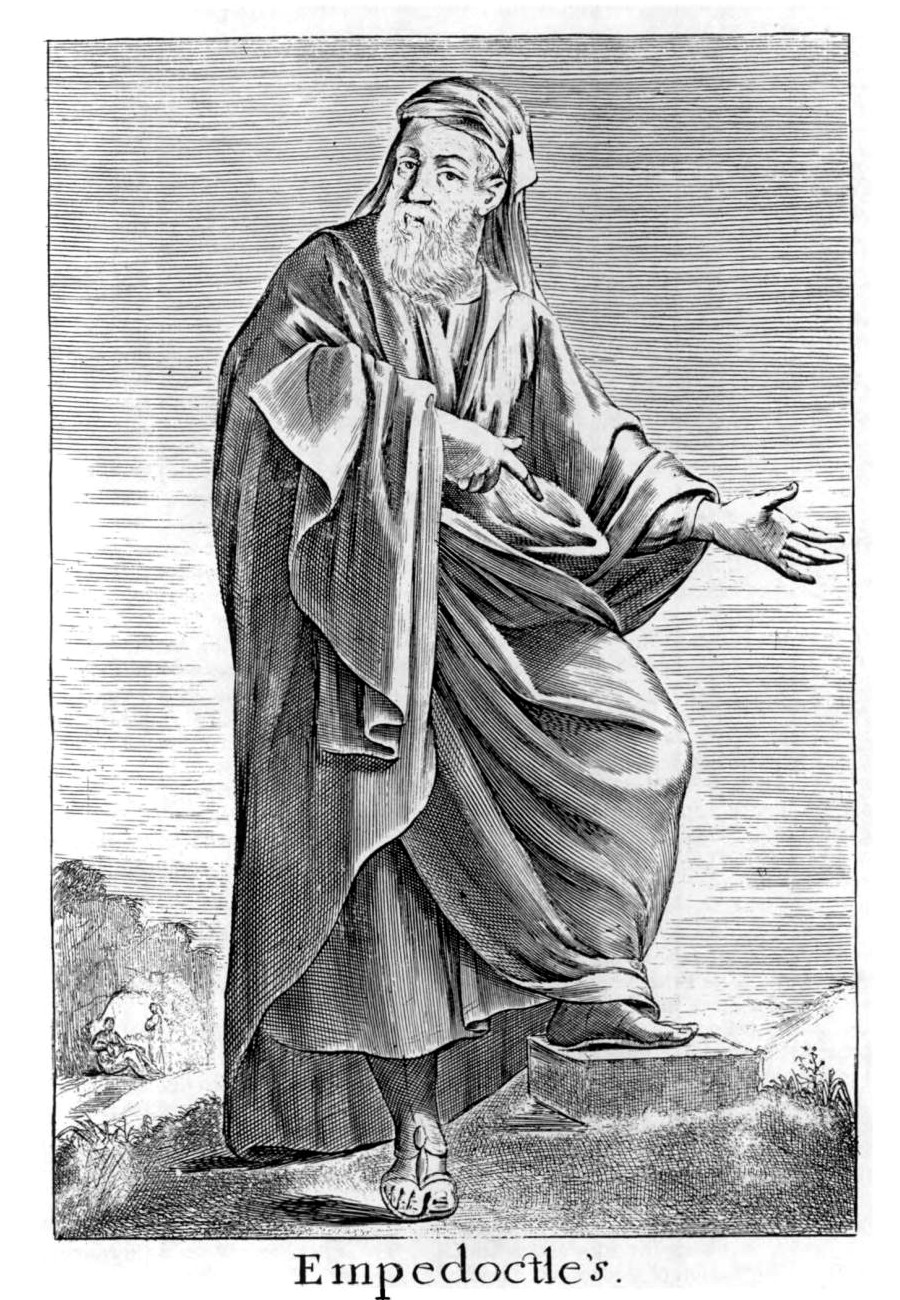
\includegraphics[width=0.7\linewidth]{../Chapter2/fig/empedocles.jpg}
		\caption{empedocles}
		\label{fig:empedocles}
	\end{subfigure}%
	\begin{subfigure}{0.5\textwidth}
		\centering
		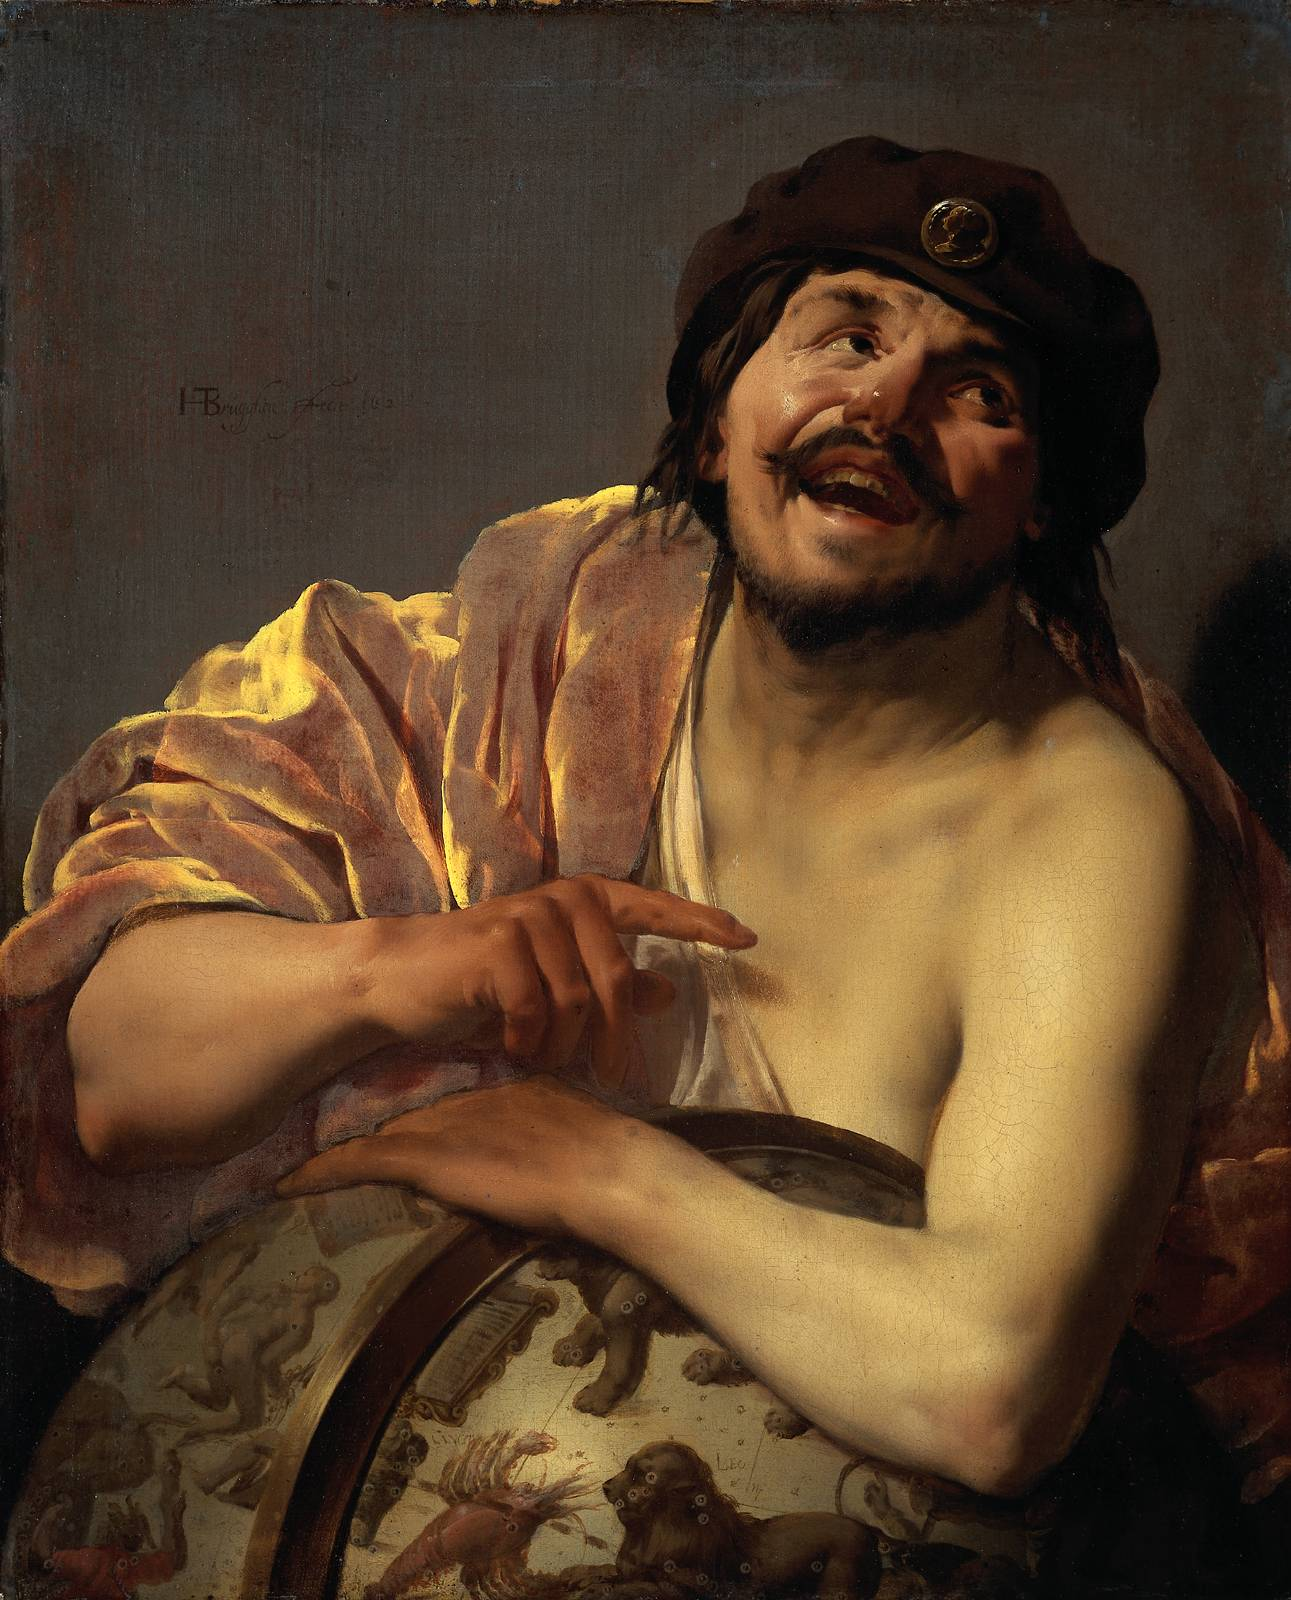
\includegraphics[width=0.7\linewidth]{../Chapter2/fig/democritus.jpg}
		\caption{Democritus}
		\label{fig:democritus}
	\end{subfigure}
	\caption{ Two greek philosophers, who made important philosophical
		contributions our understanding of matter. Empedocles (left), postulated the
		precursor to the elemental theory of matter ~\needcite{} and Democritus
		(right), postulated the precursor to the atomic theory of matter.  }
	\label{fig:atomists}
\end{figure}

Democritus was part of a movement of thought which was first to make the
intellectual jump that perhaps matter was not a continuum, but instead, composed
of 'atomon', small, indivisble particles which when configured togehter, created
all that is observable ~\needcite{}. Empedocles was making equally important
philosophical strides - in a manner complimentary to Democrits' opinion that
matter must be made of atomon, Empedocles argued that matter is composed of
elemental primatives ~\needcite{}.

Although Empedocles' 'periodic table' was only composed of Earth, Water, Fire,
and Air, the idea that some unseen transmutation of elemental forces might
generate observables in nature with quite different (but perhaps reminiscent)
properties then the 'pure substances' was an important step forward.
Proto-scientists were beginning to generate models which derived our complicated
observations, from simpler forms.

It would not be until the rise of empiricism that our means of inquiry and model
building would become sophisticated enough to ask about the make-up of the
elements themselves - protons, neutrons, electrons, and ultimately, the standard
model. 

\subsection{About 500 Years Ago...}

With the age of empiricism in full swing, scientific progress was being made at
a pace with no precident in any other period in human history~\needcite{}.

\subsection{About 200 Years Ago...}

On the shoulders of giants such as Newton and Gallileo, science finally came to
know the tool which has been indispensable to modern particle physics:
scattering.

Scattering offers a very powerful method where we one uses a well known initial
state of matter (typically in the form of a beam), allows this beam to interact
with an unknown configuration of matter, and measures the scattered beam. By
carefully studying the kinematics of the scattered beam, we can create models
which allow us to understand the structure of the target matter or describe the
nature of the interaction between the beam and target. 

Thompson
Rutherford

\subsection{Approximately Present Day}


Although Gell-Mann's simple quark model of baryons ~\needcite{} predicts the
correct quantiy for the spin of the proton, the work of Ashman et al (1988)
~\needcite{} at the European Muon Collaboraiton directly measured a portion of
the proton sturcture function $g_1$ and found that a rather small fraction of
the prton spin comes from quarks - and most of the spin is carried by the
gluons (Figure~\ref{fig:emc_g1_result}). 

\begin{figure}[H]
	\begin{center}
	
\includegraphics[width=0.5\linewidth]{../filler/squareimg.png}
	\caption{~\needfig{} ~\needcap{}. Results of EMC experiment showing that the structure
	function g1, tells us a thing about proton spin.}
	\label{fig:emc_g1_result}
\end{center}
\end{figure}

\section{Proton Spin Crisis}
\section{How to Model Proton Spin}
\begin{itemize}
		\item structure functions
		\item proton spin decomposition
		\item unpolarized parton distribution functions
		\item polarized parton distribution functions
		\item that sweet table from Delia hasch
		\item discussion $\bar{q}$, $q$, $L_q$, $g$
		\item DSSV figures
\end{itemize}
\section{How to Measure Proton Spin}
\begin{itemize}
		\item physics probes for proton spin
		\item W cross section
		\item derivation of Asymmetry
		\item kinematic extremes of Asymmetry
\end{itemize}
\subsection{Past Experimental Efforts}
\begin{itemize}
		\item summary of data on structure functions
		\item fixed target experiments
		\item collider experiments
\end{itemize}

\section{World Efforts to Measure Proton Spin}
\subsection{CERN}
\subsection{ZEUS}
\subsection{HERA}
\subsection{HERMES}
\subsection{COMPASS}
\subsection{EMC}
\subsection{SLAC}
\subsection{JLAB}

\section{Cross Sections and Luminosity}
\begin{itemize}
		\item vernier analysis note intro, equations
		\item summarize the papers on Lumoninosity
\end{itemize}
